% Full instructions available at:
% https://github.com/elauksap/focus-beamertheme

\documentclass{beamer}
\usetheme{focus}

\definecolor{main}{RGB}{92, 138, 168}
\definecolor{background}{RGB}{240, 247, 255}
%\definecolor{main}{RGB}{151, 44, 56}
%\definecolor{background}{RGB}{247, 247, 247}

%=====================define notation==================%
\usepackage{subfigure} 
\def\N{I\!\! N}
\def\R{I\!\! R}
\def\vs{\vspace{8pt}}
\def \bec{\begin{center}}
	\def \enc {\end{center}}
\def \bee {\begin{eqnarray*}}
	\def \ene {\end{eqnarray*}}
\def \no{\noindent}
\def \lo{\longrightarrow}
\def \ov{\overline}
\def \m{\multicolumn}
\def \bear{\begin{array}}
	\def \enar{\end{array}}
\def \u{\underline}
\def \bs{\begin{slide}}
	\def \es{\end{slide}}
\def \ep{\epsilon}



\def\hDash{\bot\!\!\!\bot}
\def\wh{\widehat}
\def\wt{\widetilde}
\def\ba{\mbox{\boldmath$\alpha$}}
\def\bb{\mbox{\boldmath$\beta$}}
\def\bg{\mbox{\boldmath$\gamma$}}
\def\ha{\mbox{$\widehat\ba$}}
\def\hb{\mbox{$\widehat\bb$}}
\def\hg{\mbox{$\widehat\bg$}}
\def\hDash{\bot\!\!\!\bot}


\def\a{{\bf a}}
\def\b{{\bf b}}
\def\A{{\bf A}}
\def\B{{\bf B}}
\def\C{{\bf C}}
\def\G{{\bf G}}
\def\X{{\bf X}}
\def\x{{\bf x}}
\def\Y{{\bf Y}}
\def\y{{\bf y}}
\def\Z{{\bf Z}}
\def\z{{\bf z}}
\def\u{{\bf u}}
\def\s{{\bf s}}
\def\t{{\bf t}}
\def\h{{\bf h}}
\def\k{{\bf k}}
\def\l{{\bf l}}
\def\c{{\bf c}}
\def\d{{\bf d}}
\def\w{{\bf w}}
\def\g{{\bf g}}
\def\I{{\bf I}}
\def\P{{\bf P}}
\def\Q{{\bf Q}}
\def\v1{{\bf 1}}
\def\vz{{\bf 0}}

\def\balpha{{\bm \alpha}}
\def\bbeta{{\bm \beta}}
\def\bzeta{{\bm \zeta}}
\def\betaa{{\bm \eta}}
\def\bome{{\bm \omega}}
\def\bpi{{\bm \pi}}

\def\bias{\mbox{bias}}
\def\pr{\mbox{pr}}
\def\var{\mbox{var}}
\def\cov{\mbox{cov}}
\def\cor{\mbox{cor}}
\def\MSE{\mbox{MSE}}
\def\arcos{\mbox{arcos}}

\newcommand{\trans}{^{\mbox{\tiny{T}}}}
\def\defby{\stackrel{\mbox{\textrm{\tiny def}}}{=}}

\newcommand{\beps}{\mbox{\boldmath $\varepsilon$}}
\newcommand{\bSig}{\mbox{\boldmath $\Sigma$}}
\newcommand{\hSig}{\mbox{$\widehat{\bSig}$}}
\newcommand{\bLam}{\mbox{\boldmath $\Lambda$}}
\newcommand{\hLam}{\mbox{$\widehat{\bLam}$}}
\newcommand{\bOmega}{\mbox{\boldmath $\Omega$}}
\newcommand{\bI}{\mbox{\boldmath $I$}}
\newcommand{\bGam}{\mbox{\boldmath $\Gamma$}}\def\N{I\!\! N}
\def\R{I\!\! R}
\def\vs{\vspace{8pt}}
\def \bec{\begin{center}}
	\def \enc {\end{center}}
\def \bee {\begin{eqnarray*}}
	\def \ene {\end{eqnarray*}}
\def \no{\noindent}
\def \lo{\longrightarrow}
\def \ov{\overline}
\def \m{\multicolumn}
\def \bear{\begin{array}}
	\def \enar{\end{array}}
\def \u{\underline}
\def \bs{\begin{slide}}
	\def \es{\end{slide}}
\def \ep{\epsilon}


\def\hDash{\bot\!\!\!\bot}
\def\wh{\widehat}
\def\wt{\widetilde}
\def\ba{\mbox{\boldmath$\alpha$}}
\def\bb{\mbox{\boldmath$\beta$}}
\def\bg{\mbox{\boldmath$\gamma$}}
\def\ha{\mbox{$\widehat\ba$}}
\def\hb{\mbox{$\widehat\bb$}}
\def\hg{\mbox{$\widehat\bg$}}
\def\hDash{\bot\!\!\!\bot}


\def\a{{\bf a}}
\def\b{{\bf b}}
\def\A{{\bf A}}
\def\B{{\bf B}}
\def\C{{\bf C}}
\def\G{{\bf G}}
\def\X{{\bf X}}
\def\x{{\bf x}}
\def\Y{{\bf Y}}
\def\y{{\bf y}}
\def\Z{{\bf Z}}
\def\z{{\bf z}}
\def\u{{\bf u}}
\def\s{{\bf s}}
\def\t{{\bf t}}
\def\h{{\bf h}}
\def\k{{\bf k}}
\def\l{{\bf l}}
\def\c{{\bf c}}
\def\d{{\bf d}}
\def\w{{\bf w}}
\def\g{{\bf g}}
\def\I{{\bf I}}
\def\P{{\bf P}}
\def\Q{{\bf Q}}
\def\v1{{\bf 1}}
\def\vz{{\bf 0}}

\def\balpha{{\bm \alpha}}
\def\bbeta{{\bm \beta}}
\def\bzeta{{\bm \zeta}}
\def\betaa{{\bm \eta}}
\def\bome{{\bm \omega}}
\def\bpi{{\bm \pi}}

\def\bias{\mbox{bias}}
\def\pr{\mbox{pr}}
\def\var{\mbox{var}}
\def\cov{\mbox{cov}}
\def\cor{\mbox{cor}}
\def\MSE{\mbox{MSE}}
\def\arcos{\mbox{arcos}}

\def\defby{\stackrel{\mbox{\textrm{\tiny def}}}{=}}



\title{Online Surrogate Measures \\and its Application to\\ Transportation Safety Analysis }
%\subtitle{Subtitle}
\author{Yilin Zhang}
%\author{Author 1\texorpdfstring{\\}{,} Author 2}
%\titlegraphic{
\includegraphics[scale=0.4]{ruc_logo1.png}}
%\logo{
\includegraphics[scale=0.3]{ruc_logo1.png}}
\newcommand{\nologo}{\setbeamertemplate{logo}{}}
%\institute{Institute Name \\ Institute Address}
\date{\today}

% Footline info is printed only if [numbering=fullbar].
%\footlineinfo{Custom footline text}

\begin{document}
    \begin{frame}
        \maketitle
    \end{frame}
    
    % Use starred version (e.g. \section*{Section name})
    % to disable (sub)section page.
\nologo{
	\section{Background}
    %\subsection{Subsection 1.1}
    \begin{frame}{Background}
    	\begin{itemize}
    		\item Traffic crashes are rare events, with an average rate of \alert{one crash 6.8 per million} vehicle
    		miles traveled in the US. 
    		\item The \textbf{naturalistic driving study} (NDS) provides an unprecedented
    		opportunity to evaluate crash risk.
    		\item \textbf{Second Strategic Highway Research Program} (SHRP2) NDS, the largest NDS to-date, with more than \alert{3,400 participants} and \alert{1 million hours}
    		of continuous driving data. 
    		\item The entire dataset comprised of about \alert{2000 traffic crashes}, about \alert{8000 near crashes}, and tons of thousands of \alert{normal driving segments}.
    	\end{itemize}        
    \end{frame}


    \begin{frame}{Surrogate measure}
    A broad spectrum of studies investigate identification and development of various \alert{surrogate measures}, which helps to  enhance the reliability of safety analysis.
    
    ~\\
    Our core concern is to propose surrogates based on three-dimension of acceleration.
	  \begin{itemize}
		\item Propose  \alert{new surrogate measures} to predict the risk for crash
		\item Implement the surrogate measures with  \alert{online version}
	 \end{itemize}        
   \end{frame}
    
    \begin{frame}{Data}
   		\begin{figure}[htbp]
   			\centering
   			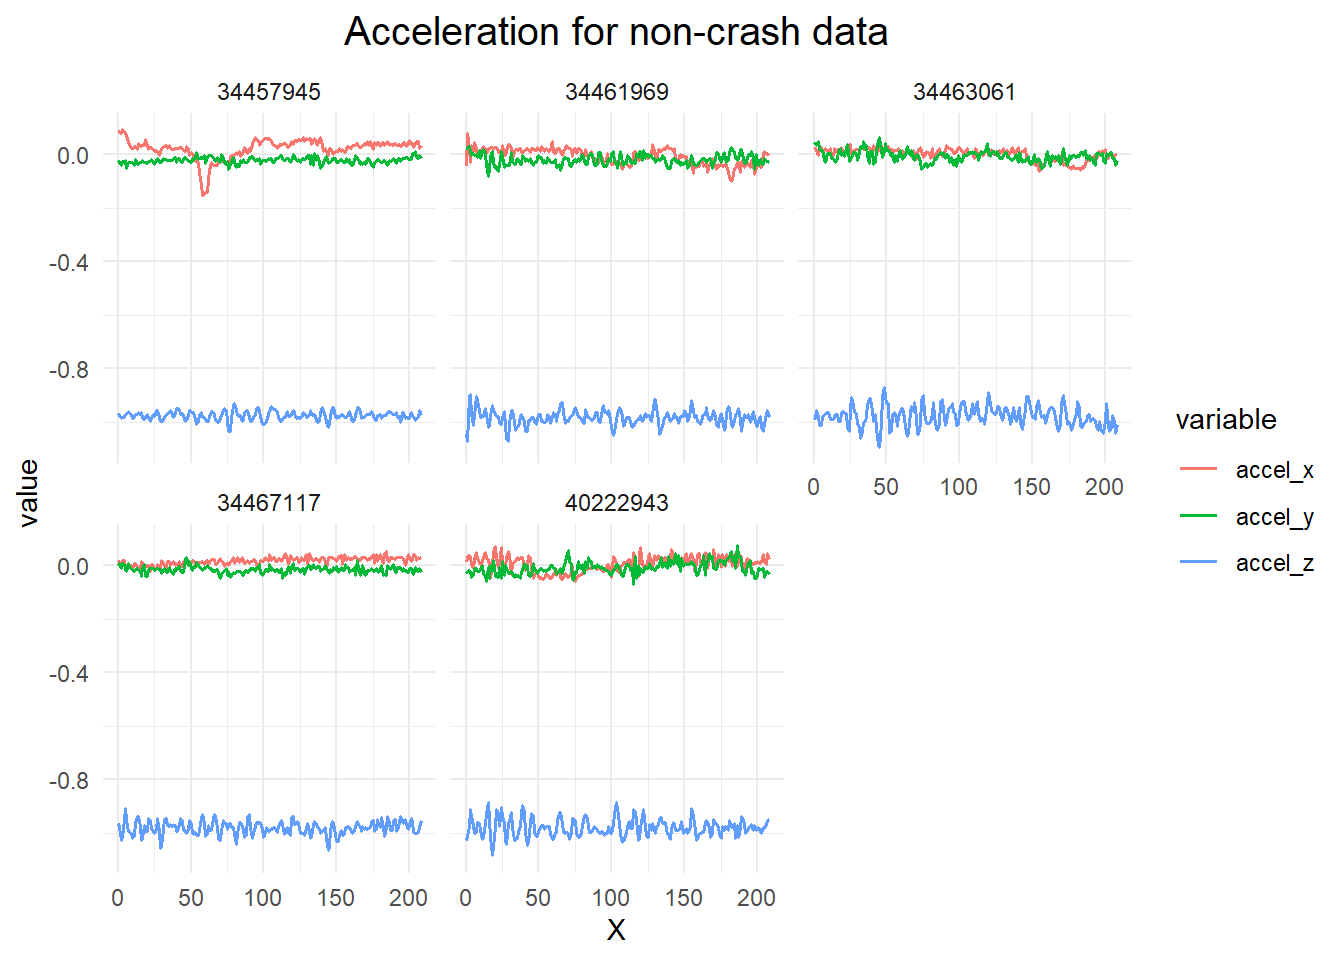
\includegraphics[width=3.5in]{figs/non_seg}
   			%\caption{Crash segment}
   			\label{fig_non_seg}
   		\end{figure}      
   \end{frame}
   
   \begin{frame}{Data}
   	\begin{figure}[htbp]
   		\centering
   		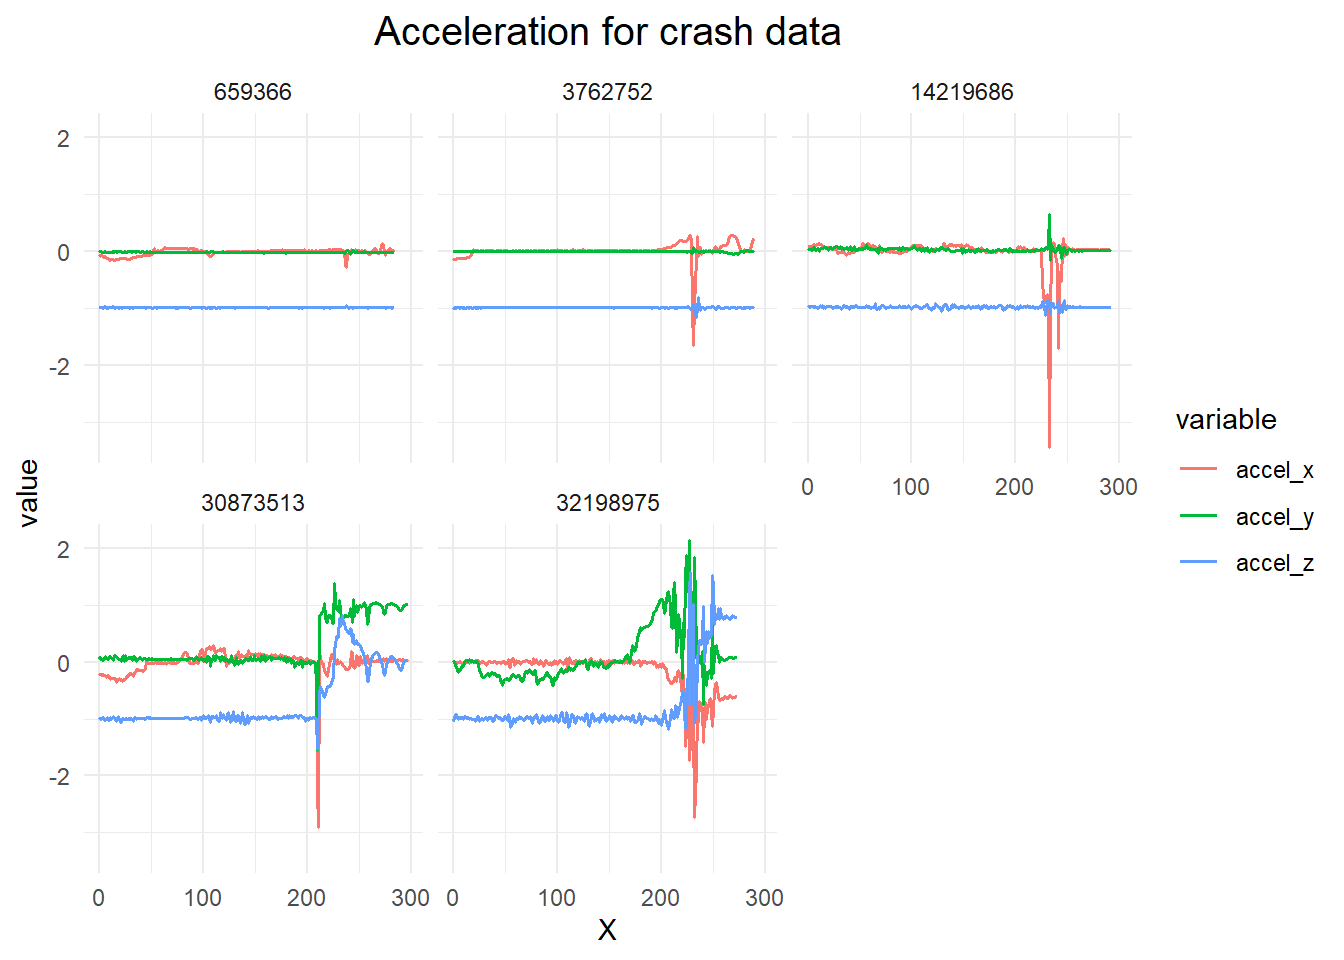
\includegraphics[width=3.5in]{figs/crash_seg}
   		%\caption{Crash segment}
   		\label{fig_crash_seg}
   	\end{figure}      
   \end{frame}

  \begin{frame}{Data}
  \alert{Trainging Data}: Each driving segment is about 200 time points, 60000 no risk segments and 1000 risky segments.
  
  ~\\
  \alert{Testing Data}:
  Each driving trip is about 2000 time points, 500 no risk trip and 100 risky trips.
     
  \end{frame}

\section{Surrogates and online estimates}
    \begin{frame}{Surrogate Measure}
   	We propose three surrogates that can be estimated via U statistics. 
   	\begin{itemize}
   		\item \alert{Standard deviation}  measures variation of the distribution.
   		\item \alert{Coefficient of Variation} (CV) measures dispersion after standardization.
   		\item \alert{Skewness} measures asymmetry of the distribution. 
   	\end{itemize}        
   \end{frame}



   \begin{frame}{Online estimation}
   	Data $\{X_i\}_{i=1}^{N}$ flow in our machine in batch.
   	\begin{itemize}
   		\item Initially, we only have $\{X_i\}_{i=1}^{n}$ data in the memory
   		\item For each time, $r$ new samples are updated in the memory, replacing those oldest $r$ ones
   	\end{itemize}   
   
    ~\\     
    \textbf{Online U statistics} 
   
    \alert{Step 1:}  We calculate the U statistics based on all initial data, which is 
    	\bee
    	\wh\theta^{(0)} \defby \binom{n}{m}^{-1}\sum_{ \{i_1,\ldots,i_m\}\in I_0} h(X_{i_1},\ldots,h_{i_m}).
    	\ene
      
   \end{frame}

   \begin{frame}{Online estimation}
   \alert{Step 2:} 
   To refresh the U statistics in time $t$, we use the following iterative formula. 
   		\bee
   		R^{(t)} &\defby& \sum\limits_{\{i_1,\ldots,i_m\}\in I_t}h(X_{i_1},\ldots,X_{i_m}) , \\
   		C^{(t)} &\defby& \sum_{k=1}^{m-1}\sum\limits_{\{i_1,\ldots,i_k\}\in J_{t-1}, \{i_{k+1},\ldots,i_m\}\in I_{t}}h(X_{i_1},\ldots,X_{i_m}) \textrm{ and } \\
   		\wh\theta^{(t)} &\defby& \left[\left\{t\binom{n}{m}-(t-1)\binom{n-r}{m}\right\}\wh\theta^{(t-1)} + C^{(t)} + R^{(t)}\right]\\
   		&&\left\{(t+1)\binom{n}{m}-t\binom{n-r}{m}\right\}^{-1}.
   		\ene
   	\alert{Step 3:} By transforming $\wh\theta^{(t)}$ as $T(\wh\theta^{(t)})$, we derive the new estimates for $T(\theta)$.         
   \end{frame}

   \begin{frame}{Online estimation}
   	To derive the asymptotic properties for $\wh\theta^{(t)}$, we denote $N_t\defby n + rt$, which is the sample size at time $t$. Then we can derive the \alert{asymptotic normality} for our online estimates.
   	\begin{block}{Theorem 1}
   		Given $E\{h(X_{1},\ldots,X_{m})\}^2<\infty$ and $\zeta_1>0$, we have
   		\bee
   		N_t^{1/2}\{T(\wh\theta^{(t)}) - T(\theta) \} \stackrel{d}{\to}\text{Normal }(0, m\zeta_1),
   		\ene
   		as $N_t$ goes to infinity.
   	\end{block} 
   \end{frame}
   
   \section{Risk prediction}
   \begin{frame}{Three surrogate measures}
    We here depict three violin of box plots for \alert{standard deviation}, \alert{coefficient of variation} and \alert{skewness}.
    \begin{figure}[htbp]
    	\centering
        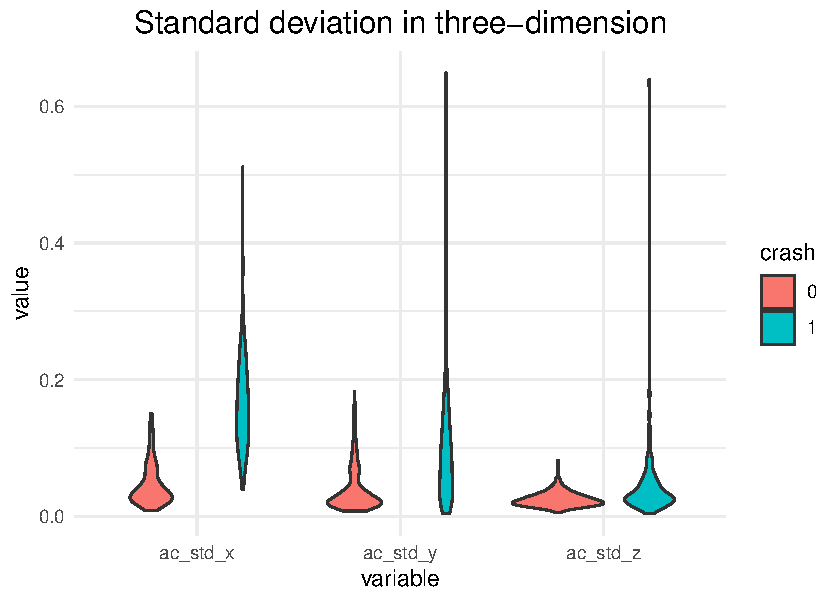
\includegraphics[width=3.0in]{figs/fig_std}
    	\label{fig_std}
    \end{figure}
   \end{frame}

   \begin{frame}{Three surrogate measures}
    	\begin{figure}[htbp]
    		\centering
    		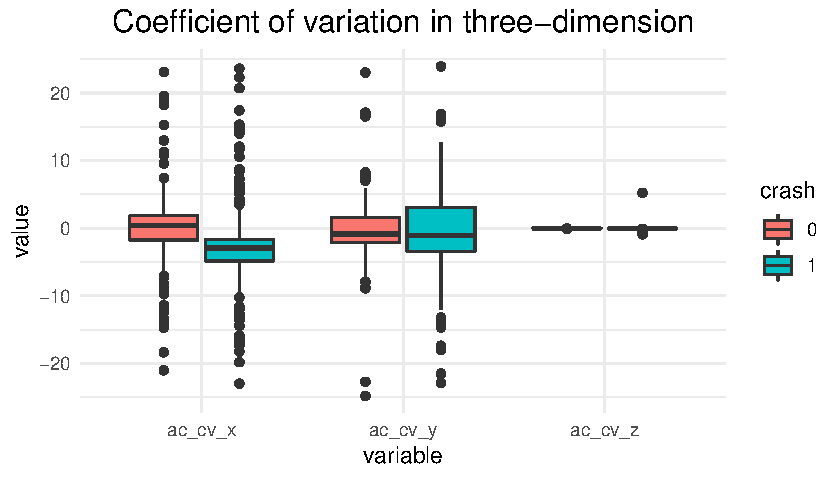
\includegraphics[width=3.0in]{figs/fig_cv}
    		\label{fig_std}
    	\end{figure}
    \end{frame}

    \begin{frame}{Three surrogate measures}
    	\begin{figure}[htbp]
    		\centering
    		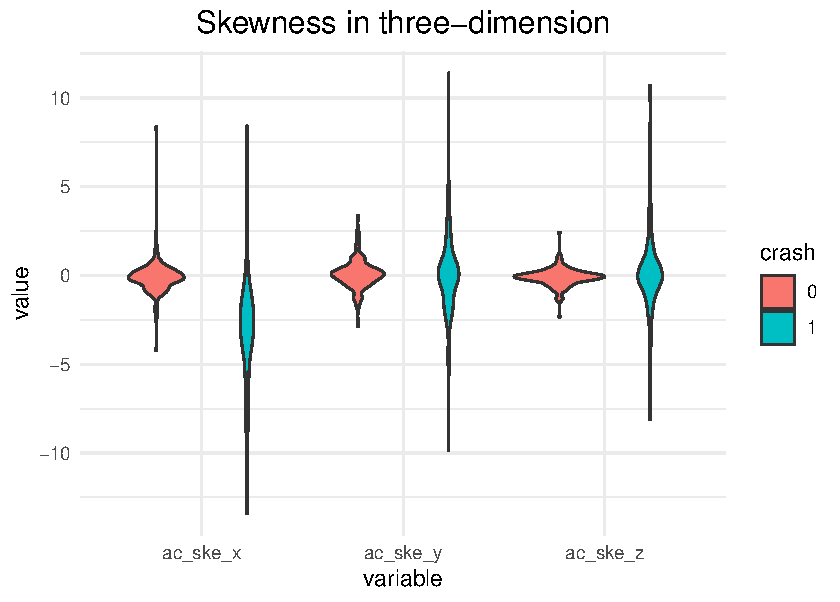
\includegraphics[width=3.0in]{figs/fig_ske}
    		\label{fig_std}
    	\end{figure}
    \end{frame}
    
    
    \begin{frame}{Prediction model}
     We build the prediction model based on training and testing steps.
     
     ~\\
     
     \textbf{Training step:} Build the benchmark model.
     \begin{itemize}
     	\item Three surrogates with dimensions are input
     	\item The safety benchmark model consists 61000 driving segments
     	\item Each driving segment is about 200 time points
     	\item 60000 baselines and 1000 crash
     	\item Train a GBDT model as a safety benchmark model
     \end{itemize}
    \end{frame}

    \begin{frame}{Prediction model}

    	\textbf{Prediction step:} Predict use online estimation.
    	\begin{itemize}
    		\item Each driving trip is about 2000 time points, 500 no risk trip and 100 risky trips
    		\item Initial with 200 time points and 50 time points renew each time
    		\item Using the online estimation to extract features for every trip
    		\item Then use the safety benchmark model to estimate timely risk
    	\end{itemize}
    \end{frame}


    \begin{frame}{Prediction model}
    	\begin{figure}[htbp]
    		\centering
    		\subfigure[Lateral]{
    			\begin{minipage}[t]{0.5\linewidth}
    				\centering
    				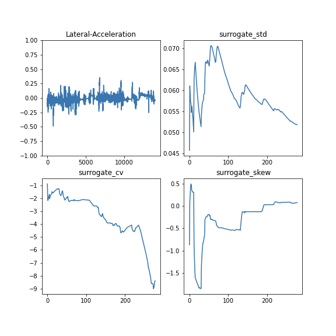
\includegraphics[width=2.2in]{figs/later_ac_non}
    				%\caption{fig2}
    			\end{minipage}
    		}%
    		\subfigure[Longitudinal]{
    			\begin{minipage}[t]{0.5\linewidth}
    				\centering
    				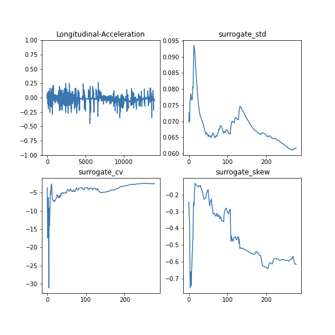
\includegraphics[width=2.2in]{figs/long_ac_non}
    				%\caption{fig2}
    			\end{minipage}%
    		}%
    		\centering
    		\caption{Online estimation for non-crash trip}
    		\label{fig_non_trip}
    	\end{figure}
    \end{frame}


     \begin{frame}{Prediction model}
    	\begin{figure}[htbp]
    		\centering
    		\subfigure[Lateral]{
    			\begin{minipage}[t]{0.5\linewidth}
    				\centering
    				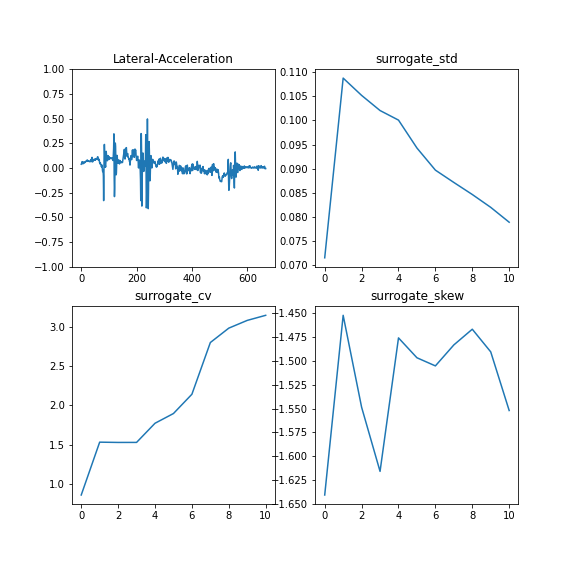
\includegraphics[width=2.2in]{figs/later_ac_crash}
    				%\caption{fig2}
    			\end{minipage}
    		}%
    		\subfigure[Longitudinal]{
    			\begin{minipage}[t]{0.5\linewidth}
    				\centering
    				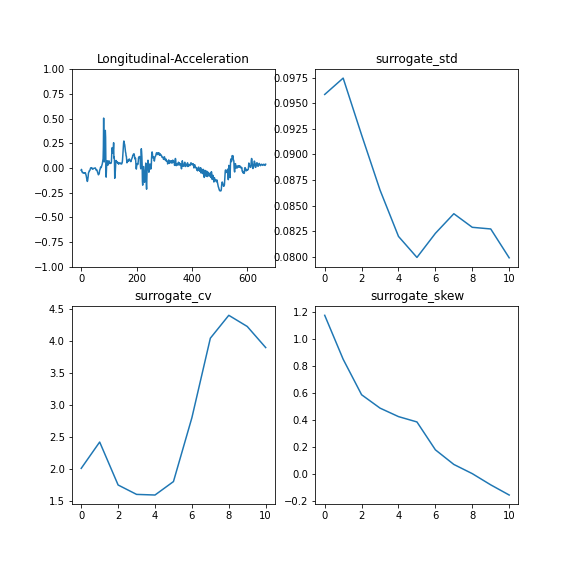
\includegraphics[width=2.2in]{figs/long_ac_crash}
    				%\caption{fig2}
    			\end{minipage}%
    		}%
    		\centering
    		\caption{Online estimation for crash trip}
    		\label{fig_crash_trip}
    	\end{figure}
    \end{frame}
    

    \begin{frame}{Prediction model}	
    	\textbf{Evaluation:} We average online risk during a trip and depict box-plots for  crash and non-crash trip.
        \begin{figure}[htbp]
        	\centering
        	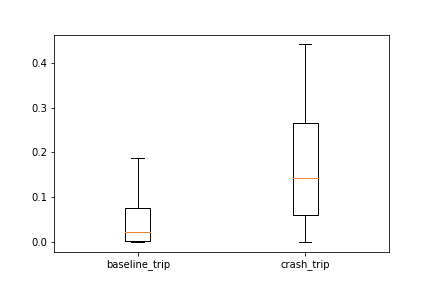
\includegraphics[width=3.0in]{figs/risk_box}
        	\label{fig_box}
        \end{figure}
    \end{frame}
    
    
    \section{Further work}
     \begin{frame}{Further work}	
        \begin{enumerate}
        	\item More prediction models will be considered.
        	\item Old methods comparisons for example, maximum of acceleration
        	\item Robustness of model
        \end{enumerate}
    \end{frame}

    \begin{frame}[focus]
        \textbf{Thanks for Listening !}
    \end{frame}
    }


\end{document}
